\vspace{-2cm}
\begin{columns}[t,totalwidth=\twocolwid] % Split up the two columns wide column
		
		\begin{column}{0.5\twocolwid}%\vspace{-.6in} % The first column within column 2 (column 2.1)
        \vspace{2cm}
  		\centering
			\begin{figure}
                 \captionbox
                 {Attitude control on the quadcopter. The first part of the figure shows how the angles are stabilized, then, a reference in roll of 0.4 rad is given to the controller while the other angles remain at zero.}
				{
                    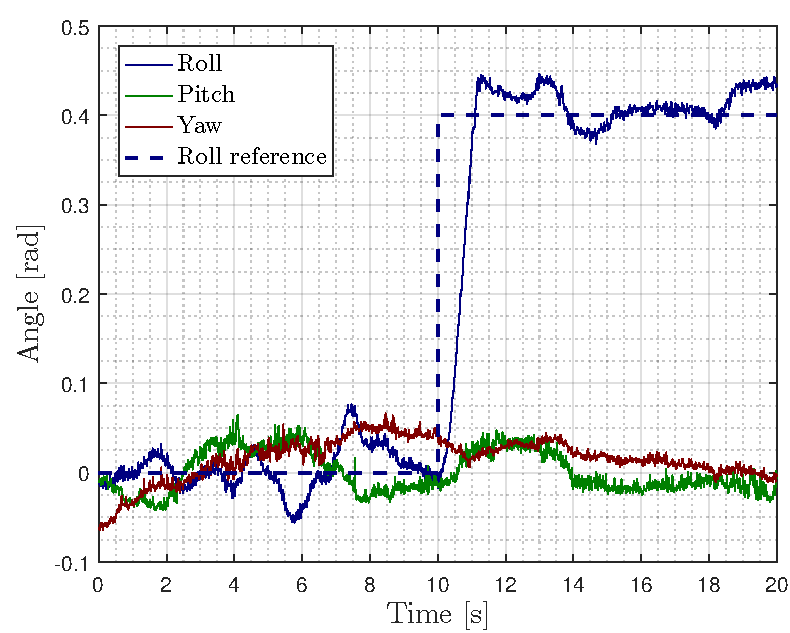
\includegraphics[width=.9\linewidth]{figures/AttitudeControl}
				}
			\end{figure}
		\end{column} % End of column 2.1
		
		\begin{column}{0.5\twocolwid}%\vspace{-.6in} % The second column within column 2 (column 2.2)
			\begin{figure}[H]
			\hspace{-6cm}
			    \captionbox  %<--use captionbox instead if no global caption is needed
			    {The translational controllers tracking a helical trajectory. The network is included in all simulations.}
			    {
			      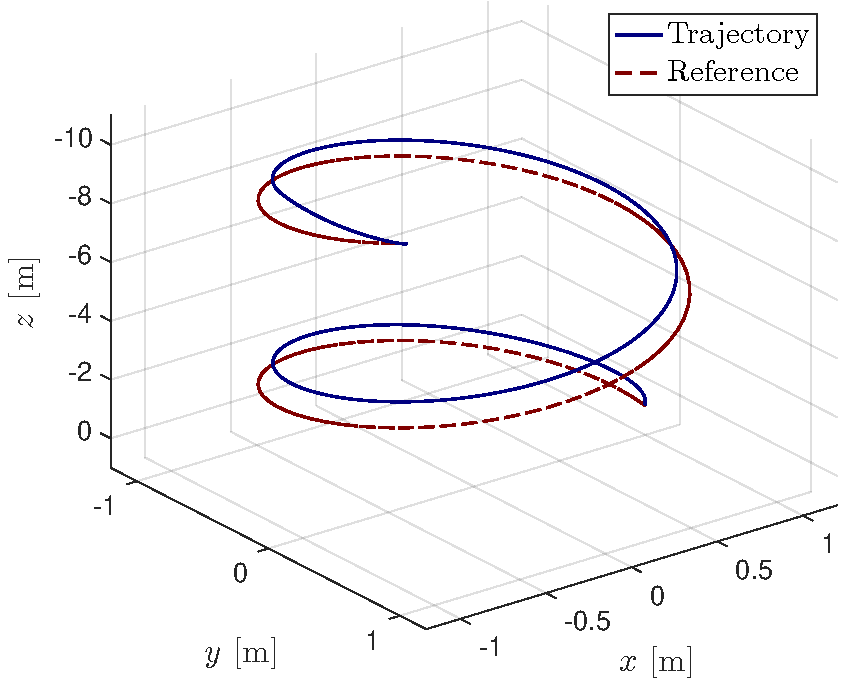
\includegraphics[width=.69\textwidth]{figures/helix}
			    }
			\end{figure}
			\vspace{-1cm}
			\begin{figure}[H]
			\hspace{-2cm}
			    \captionbox
			    {Step responses of the translational position controllers in simulation.} 
			    {
			      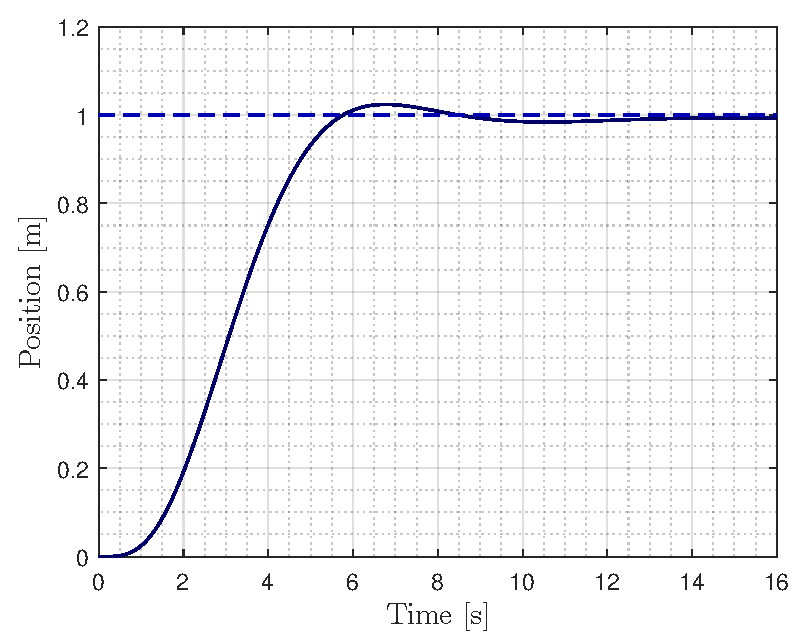
\includegraphics[width=.29\textwidth]{figures/xStep}
			      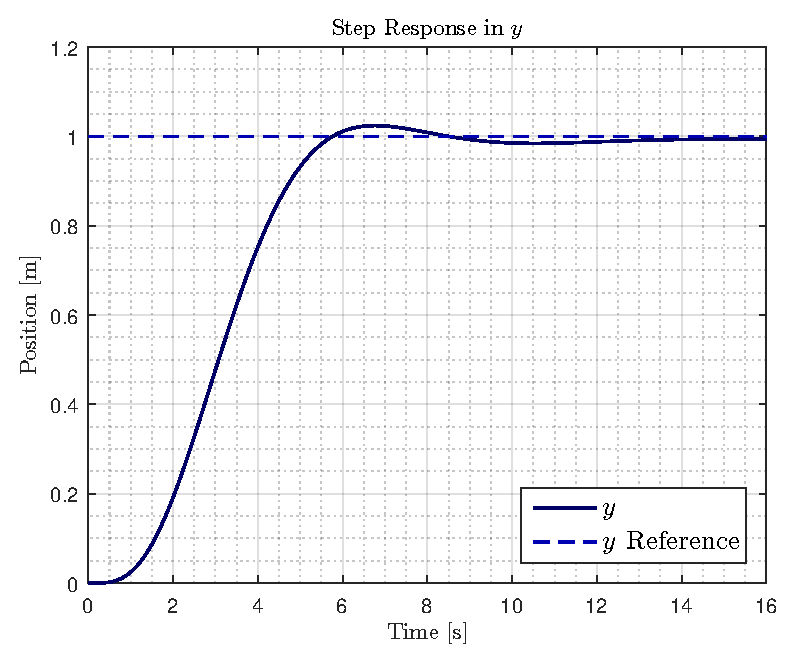
\includegraphics[width=.29\textwidth]{figures/yStep}
			      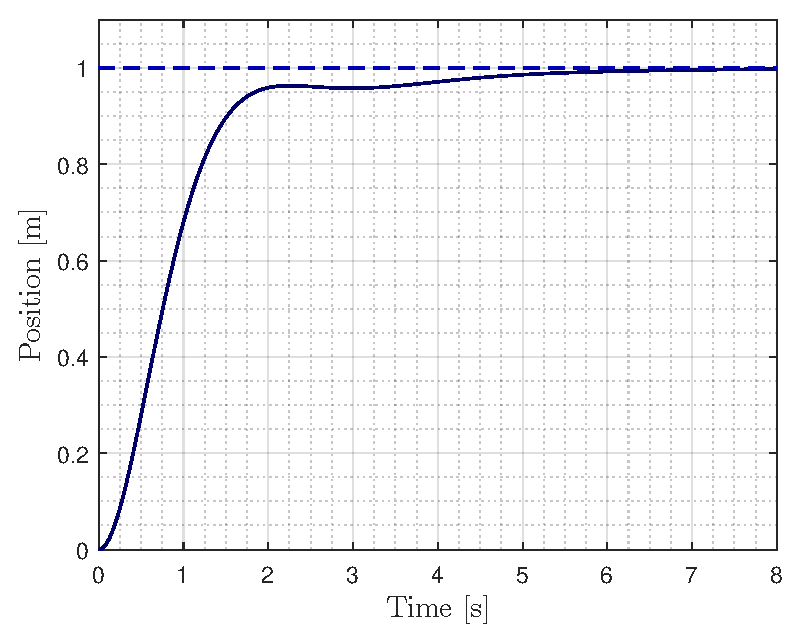
\includegraphics[width=.29\textwidth]{figures/zStep}
			    }
			\end{figure}
		\end{column} % End of column 2.2
		
	\end{columns} % End of the split of column 2 - any content after this will now take up 2 columns width